\chapter{Fundamentação Teórica}

\section{Modelagem de Processos}

A dinâmica de muitos sistemas mecânicos, elétricos, térmicos, econômicos, biológicos ou outros pode ser descrita em termos de equações diferenciais. Estas equações são obtidas pelas leis físicas que regem dado sistema, por exemplo, as leis de Newton para sistemas mecânicos e as leis de Kirchhoff para sistemas elétricos. Um só modelo matemático, no entanto, não é o único para determinado sistema, pois ele pode ser representado por muitas maneiras diferentes e, portanto, por vários modelos matemáticos, dependendo da perspectiva a ser considerada. \cite{katsuhiro2010}

Uma das formas mais comuns de representação de um sistema genérico é por funções de transferências. Sendo $y(t)$ a função que descreve uma saída de um processo, e $x(t)$ a de uma entrada, a função de transferência $G(s)$ traduz a influência de x em y. Assim, a função $G(s)$ advém das equações físicas descritivas de um processo e, de maneira geral se torna mais complexa quanto mais equações e parâmetros influentes são considerados. Como um exemplo, ao modelar a queda de um corpo livre, tomando como variável de saída sua posição, uma função de transferência simples consideraria apenas a influência da gravidade sobre o corpo, e a mesma pode se tornar mais complexa se considerasse o atrito e resistência com o ar.

Um processo, após modelado, pode se traduzir em um sistema linear ou não linear. Um sistema é dito linear se o princípio da superposição se aplicar a ele. Este princípio afirma que a resposta produzida pela perturbação simultânea de duas entradas é a soma das duas respostas individuais para cada entrada. A partir deste, princípio, é possível calcular soluções complexas a partir do cálculo de cada parte que a compõe. \cite{katsuhiro2010}

Sistemas não lineares são, em geral, mais difíceis de modelar e de controlar. Para tais, podem ser empregadas algumas técnicas de trasformações em sistemas lineares equivalentes. Uma delas é a chamada linearização, que emprega a série de Taylor, truncanda no segundo termo, ou
\begin{equation}
f(x1, x2, .. , xn) \simeq f(x1_0, x2_0, ..., x3_0) + \bigg( \sum_{i=1}^n \frac{df}{dxi}\big|_{xi=xi_0} (xi - xi_0) \bigg),
\end{equation}
, obtendo assim, uma função linearizada em torno de um determinado ponto de operação do processo ($x_i$ são os parâmetros da função descritiva $f$, e ${x_i}_0$ são os pontos de operação). Quanto mais as variáveis do sistema linearizado se afastarem deste ponto de operação, maior será o erro deste sistema, em relação ao sistema gerador não linear. Outra técnica é simplesmente partir o sistema não linear com uma entrada qualquer, e pela análise do gráfico de resposta projetar um sistema linear que seja o mais fiél possível ao primeiro.

Talvez o maior benefício da modelagem de processos para o setor industrial seja a possibilidade de projetar sistemas de controle mais eficientes, eliminando a necessidade de gastar tempo e dinheiro com testes em campo. Softwares como MATLAB e GNU Octave permitem que, a partir de funções modeladoras (no tempo ou no domínio s), um processo seja parametrizado, e seu comportamento, dada entradas também configuradas, seja simulado.

\section{SCADA}

Os sistemas supervisórios podem ser considerados como o nível mais alto de IHM, pois mostram o que está acontecendo no processo e permitem ainda que se atue neste. A evolução dos equipamentos industriais, com a introdução crescente de sistemas de automação industrial, tornou complexa a tarefa de monitorar, controlar e gerenciar esses sistemas. \cite{Martins2007}

Sistemas SCADAs são responsáveis por buscar informações de controladores e equipamentos diversos de automação e manipular estas informações de diversas maneiras. As aplicações mais simples se constituem na visualização dinâmica destes dados através de objetos, mostradores, cores, entre outros meios dispostos em telas pré programadas. Uma estratégia, por exemplo, é representar todo um sistema por imagens já embutidas na biblioteca do software editor, e incluir o máximo de informações importantes referentes ao mesmo em uma única tela detalhada. Outra seria agrupar as informações por temática, e mostrar diversas telas menos detalhadas, que alternem entre si de acordo com um temporizador interno. A Figura \ref{img_supervisorio_exemplo} ilustra um exemplo de tela para um sistema supervisório.

\begin{figure}[hbt]
	\centering
	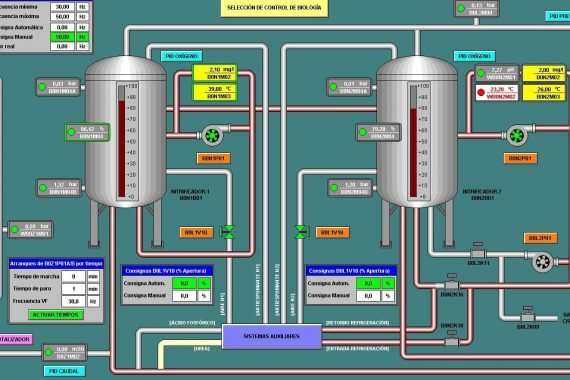
\includegraphics{Supervisorio_exemplo}
	\caption[Fonte: https://www.agaads.com/service/scada-system/]{Tela exemplo de um sistema supervisório}
	\label{img_supervisorio_exemplo}
\end{figure}

Outro emprego comum de sistemas SCADA, é de serem responsáveis por informar valores de setpoint aos controladores acoplados a um processo, os quais podem advir de um cálculo computacional ou manual, por um operador. É possível ainda o sistema ser responsável pelo controle, enviando aos atuadores conectados somente o sinal de controle. Esta estratégia, no entanto, não é recomendada, por questões de confiabilidade da transmissão de dados e velocidade de processamento.

Por ser executado geralmente em um computador comum, a palavra chave de um sistema supervisório é flexibilidade. Um sistema SCADA deve ser capaz de se comunicar por diversos protocolos com diversos dispositivos, e adicionalmente disponibilizar os valores lidos para outros usuários, não somente os que têm acesso às telas. Por possuir esta funcionalidade, software SCADAs ultrapassam o nível 2 na pirâmide de automação (Figura \ref{img_piramide_automacao}), chegando ao nível de supervisão da produção, pois agrupa as informações de diversos controladores e sensores em um só local, gerando suporte para ações de gerência.

\begin{figure}[hbt]
	\centering
	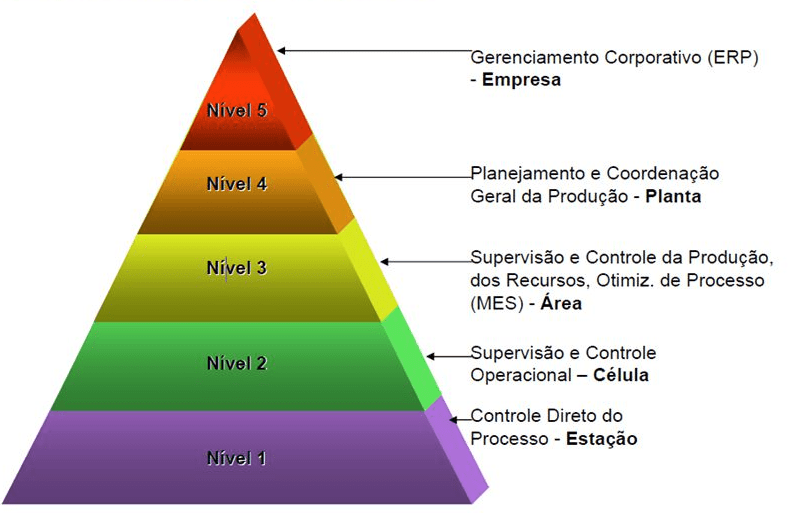
\includegraphics[width=0.8\textwidth]{piramide_automacao}
	\caption[Fonte: https://www.logiquesistemas.com.br/blog/piramide-de-automacao-industrial/attachment/354/]{Pirâmide da automação}
	\label{img_piramide_automacao}
\end{figure}

A fim de atingir uma maior compatibilidade com programas e usuários externos, a maior parte dos softwares supervisórios permitem de forma simples a criação de um banco de dados para os valores monitorados. Os mesmos podem ser exportados em forma de relatórios em layouts já embutidos e utilizados como insumos para tomada de decisões e cálculo de performance.

Segundo \cite{Roggia2016}, dentre os principais benefícios do uso de sistemas de supervisão podem-se citar: informações instantâneas, redução no tempo de produção, redução no custo de produção, precisão das informações, detecção de falhas, aumento da qualidade e aumento da produtividade.

\section{Comunicação Serial}

Comunicação serial é um meio simples de dois equipamentos trocarem informação em formato de uma série de bits. De acordo com \cite{Bolton2015}, ela se dá através de um único cabo ou pino, transmitindo apenas um bit de cada vez. Apesar disto significar uma velocidade menor de envio de dados, a comunicação serial possui baixo custo, sendo popularmente utilizada na transmissão de dados por longas distâncias.Ainda existem outras tecnologias, como a chamada comunicação paralela, que utilizam mais canais de comunicação e podem portanto transmitir vários bits simultaneamente.

Segundo \cite{Mazidi2016}, existem dois tipos de comunicação serial: assíncrona ou síncrona. Como sugerido por seus nomes, a comunicação síncrona transmite blocos de tamanhos definidos, em momentos definidos, enquanto que o outro tipo transmite bytes de dados em qualquer momento. Para contornar a necessidade de escrever trechos de código que lidem como os dois casos, muitos fabricantes utilizam chips de circuitos integrados que manipulam o fluxo de dados, facilitando a escrita de scripts de comunicação.

Diversos equipamentos eletrônicos utilizam a comunicação serial, como mouses e teclados. O conhecido controlador Arduino UNO também permite a troca de bits por meio de suas portas seriais, de números 0 ou 1, ou uma mais comumente utilizada entrada USB (\cite{ArduinoSerial}). Ela também está presente em alguns protocolos de comunicação modernos, como Ethernet e Profibus.

Como ilustrado na figura \ref{img_serial_comm}, e fundamentado por \cite{Mazidi2016}, um modelo de transmissão para bytes (8 bits) de informação pela porta serial se constituiria em uma onda digital cujos formato se traduz em um bits 1 ou 0. O primeiro bit marca o início da transmissão, seguido por 8 bits relativos à informação enviada, um bit opcional de paridade (acrescentado por fins de validação de dados), e um último bit que encerra o bloco de informação. Protocolos de comunicação diferentes podem acrescentar ou remover características à sequência transmitida, seja para assegurar a integridade da informação, acrescentar outras informações na cadeia, ou para aumentar a velocidade de comunicação.

\begin{figure}[hbt]
	\centering
	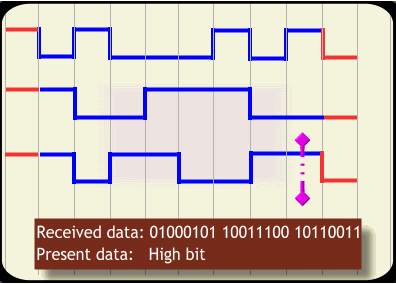
\includegraphics{serial_comm}
	\caption[Fonte: http://electrosofts.com/parallel/]{Exemplo de transmissão serial de uma sequência de 3 bytes}
	\label{img_serial_comm}
\end{figure}

Por comunicar dois equipamentos distintos, com diferentes arquiteturas, se fazem necessárias medidas que contornam a diferença entre os clocks de ambos, em outras palavras, a diferença entre a velocidade de transmissão e a de leitura dos bits recebidos. Uma delas é a utilização de um buffer, um espaço de memória na porta receptora, que guarde rapidamente os bits transmitidos, para posterior leitura e tratamento dos mesmos por parte do processador da máquina. Quando este buffer está próximo de encher, o receptor pode fechar o barramento serial via hardware ou software, para impedir a perda de informação durante sua transmissão.

Em seu artigo, \cite{Denver1995} sugere o emprego de threads para contornar possíveis problemas na comunicação serial, como a espera para receber valores. Neste caso, threads impediriam que toda uma aplicação parasse até que a transmissão deste valor seja completada. 

\section{Qt em Python}

Segundo seu criador, \ref{Rossum2003}, Python foi criada no início da década de 90, com influências de outra linguagem na qual trabalhara, chamada ABC. O objetivo do projeto ABC era de criar uma linguagem que pudesse ser ensinada à usuários inteligentes de computadores, mas que não eram programadores nem desenvolvedores de softwares. Após ingressar em outro projeto, surgiu a necessidade de implementação de outra linguagem, onde Rossum teve a iniciativa de criar o Pyhton: uma  linguagem simples e escalável, que permitisse a contribuição de terceiros.

Se tratando de sua arquitetura, Python é uma linguagem de alto nível, orientada a objetos e com tipagem dinâmica e forte. As definições de escopo e blocos de código são representadas por indentações, o que torna o código mais organizado e visualmente aprazível, dispensando a utilização de chaves para delimitar escopo. Além disto, permite interoperabilidade com outras linguagens. Por exemplo, utilizando a ferramenta Cython é possível, a partir de um código Python, gerar um código equivalente em C. Existem funções, inclusive, que são desenvolvidas em C, a fim de agilizar o processamento de grandes bases de dados, mas implementadas em Python.

No âmbito acadêmico, Python apresenta boas vantagens. Não só é considerada simples fácil de aprender, como é gratuita e open source. Logo, seus usuários e clientes não têm custos com licenças e seus desenvolvedores podem usar livremente códigos publicados por terceiros, que geralmente se apresentam de fácil acesso na internet, e adaptá-los às suas necessidades. Em uma enquete realizada pelo conhecido fórum da comunidade de computação Stack Overflow, Python foi considerada a 3ª “linguagem mais amada” pelo público.

Pela facilidade de compartilhamento e comunidade crescente de usuários, existem diversas bibliotecas úteis de Python que podem ser baixadas diretamente de um repositório online e facilmente instaladas. Como alguns exemplo, cita-se as libs SQLAlchemy, que permite criação e acesso a bancos de dados leves; NumPy, uma poderosa ferramenta para cálculos matriciais; e PyQt5, que possui objetos e métodos para criação de interfaces gráficas.

Segundo sua documentação \cite{QT2020}, a biblioteca PyQt5 veio da biblioteca de C++ “Qt”, que implementa APIs para outras linguagens, permitindo-as implementar seus objetos em seus códigos. No seu site oficial, existe uma documentação extensa de todos os seus objetos em C++, e existem também muitos exemplos disponíveis online, tanto em sites oficiais do Qt como em fóruns de programadores.

Existem 3 módulos do PyQt julgados principais para criação de GUIs locais:

\begin{itemize}
	\item QtWidgets: Engloba os objetos gráficos principais, como botões, textos e layouts. O objeto genérico QWidget, herdado por diversos outros deste módulo, tem funções cruciais relativas ao posicionamento, geometria, visibilidade e estilo dos objetos gráficos.
	\item QtCore: Este módulo lida com eventos dos objetos da GUI, como cliques de botões e edições de caixas de texto, e conecta estes eventos com funções definidas pelo programador. Ele também permite que ele configure a aplicação principal e coordena possíveis threads iniciadas por ela.
	\item QtGui: Contém objetos que possibilitam a edição de cores e bordas dos Widgets e também lida com eventos relacionados à atualização da posição e estética destes objetos.
\end{itemize}

Para iniciar a GUI, deve ser criado um objeto \emph{QApplication}, que representa o núcleo da aplicação, juntamente com as janelas da mesma, que são objetos \emph{QMainWindow}. Estes aceitam um objeto genérico \emph{QWidget} como Widget central principal (através do método \emph{setCentralWidget()}), cujas características de tamanho e layouts internos definem o tamanho da janela. Inicia-se a aplicação pelo comando \emph{exec\_()}, e as janelas pelo comando \emph{show()}.

Numa interface criada com PyQt5, os objetos visíveis dispostos na tela são chamado de Widgets, e herdam da classe \emph{QWidget}. Por conta da arquitetura em objetos da biblioteca, uma boa prática para programadores é colocar um Widget dentro do outro, no sentido de design e posicionamento. Assim, é possível definir melhor o espaço e as condições de redimensionamento dos objetos quando a janela for esticada ou comprimida, pois cada layout redimensionará apenas os Widgets que contém, dentro do espaço disponível.

A Figura \ref{img_exemplo_qwidget} ilustra a organização padrão de uma aplicação em PyQt, listando também alguns objetos populares.

\begin{figure}[hbt]
\centering
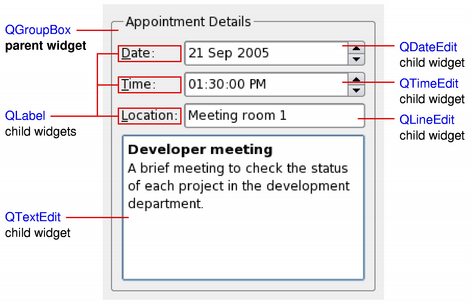
\includegraphics{Exemplo_QWidget}
\caption[Fonte: https://doc.qt.io/qt-5/qwidget.html]{Janela \emph{QMainWindow} com um \emph{QGroupBox} como Widget central, contendo vários outros Widgets em um layout \emph{QGridLayout} dentro de outro layout \emph{QHBoxLayout}}
\label{img_exemplo_qwidget}
\end{figure}
